\chapter{Hadoop}
\label{cap:hadoop}

Este capítulo irá discutir sobre o software Hadoop.

\section{Hadoop Distributed File System}

Quando uma base de dados atinge a capacidade máxima de espaço provida por uma única máquina física, torna-se necessário distribuir esta responsabilidade com um determinado número de computadores. Sistemas que gerenciam o armazenamento de arquivos em uma ou mais máquinas interligadas em rede são denominados sistemas de arquivos distribuídos. Como seu funcionamento depende dos protocolos de rede que serão utilizados, todos os problemas relacionados a própria rede tornam-se inerentes a este tipo de abordagem, adicionando uma complexidade muito maior aos sistemas de arquivos distribuídos, como por exemplo, em relação aos sistemas de arquivos convencionais.

No contexto de Big Data, que engloba um volume muito grande de dados, a utilização de um mecanismo para armazenar informações ao longo de várias máquinas é indispensável. Neste sentido a camada mais baixa do Hadoop é composta por um sistema de arquivos distribuídos chamado Hadoop Distributed File System (HDFS). Apesar de apresentar semelhanças com os sistemas de arquivos distribuídos existentes seu grande diferencial está na alta capacidade de tolerância a falhas, no baixo custo de hardware que é requerido e também na alta escalabilidade.

\subsection{Principais Características}

O HDFS foi projetado para armazenar arquivos muito grandes a uma taxa de transmissão de dados constante, sendo executado em clusters com hardware de baixo custo2. Suas principais características de design podem ser descritas a seguir:

\begin{enumerate}

\item Arquivos muito grandes: Este sistema de arquivos distribuídos é capaz de armazenar arquivos  que chegam a ocupar terabytes de espaço, portanto é utilizado por aplicações que necessitam de uma base de dados extremamente volumosa. Segundo SHAVACHCKO3, Os clusters do Hadoop utilizados pelo Yahoo chegam a armazenar 25 petabytes de dados.
\item Streaming data access: Operações de leitura podem ser realizadas nos arquivos quantas vezes forem necessárias, porém um arquivo pode ser escrito apenas uma única vez. Esta abordagem pode ser descrita como “write-once, read-many-times”2, este sistema de arquivos distribuídos foi construído partindo da ideia que este modelo é o mais eficiente para processar os dados. O HDFS também realiza a leitura de qualquer arquivo a uma taxa constante, ou seja, a prioridade é garantir vazão da leitura do arquivo e não minimizar a latência ou prover interatividade com aplicações em tempo real, como é realizado em sistemas de arquivos com propósito geral.
\item Hardware de baixo custo: O HDFS foi projetado para ser executado em hardwares que não precisam ter necessariamente alta capacidade computacional e também alta confiabilidade. O sistema foi desenvolvido partindo do pressuposto que a chance dos nós ao longo do cluster falharem é extremamente alta, portanto mecanismos de tolerância a falha foram desenvolvidos para contornar este problema, permitindo uma maior flexibilidade quanto ao uso de diferentes tipos de hardwares.

\end{enumerate}


\subsection{Divisão em Blocos}

Um disco é dividido em vários blocos com tamanho fixo, os quais compõe a menor estrutura de dados, onde são realizadas escritas e leituras. Em sistemas de arquivos convencionais cada bloco não ocupa mais que alguns KB de espaço, geralmente 512 bytes, esta informação é totalmente transparente para o usuário do sistema, no qual apenas realiza operações sobre arquivos de diferentes tamanhos, nele contido.

O HDFS também possui o conceito de blocos, porém estes possuem tamanho bem maior, por padrão ocupam 64MB de espaço. Cada arquivo criado no sistema é quebrado em blocos com estas características, no qual cada um é salvo como uma unidade independente, podendo estar localizado em qualquer nó do cluster. O HDFS foi projetado para armazenar arquivos que ocupam grande quantidade de espaço em disco, portanto com blocos de tamanho elevado o tempo de busca no disco é reduzido significativamente.


\begin{figure}[h!]
	\centering
	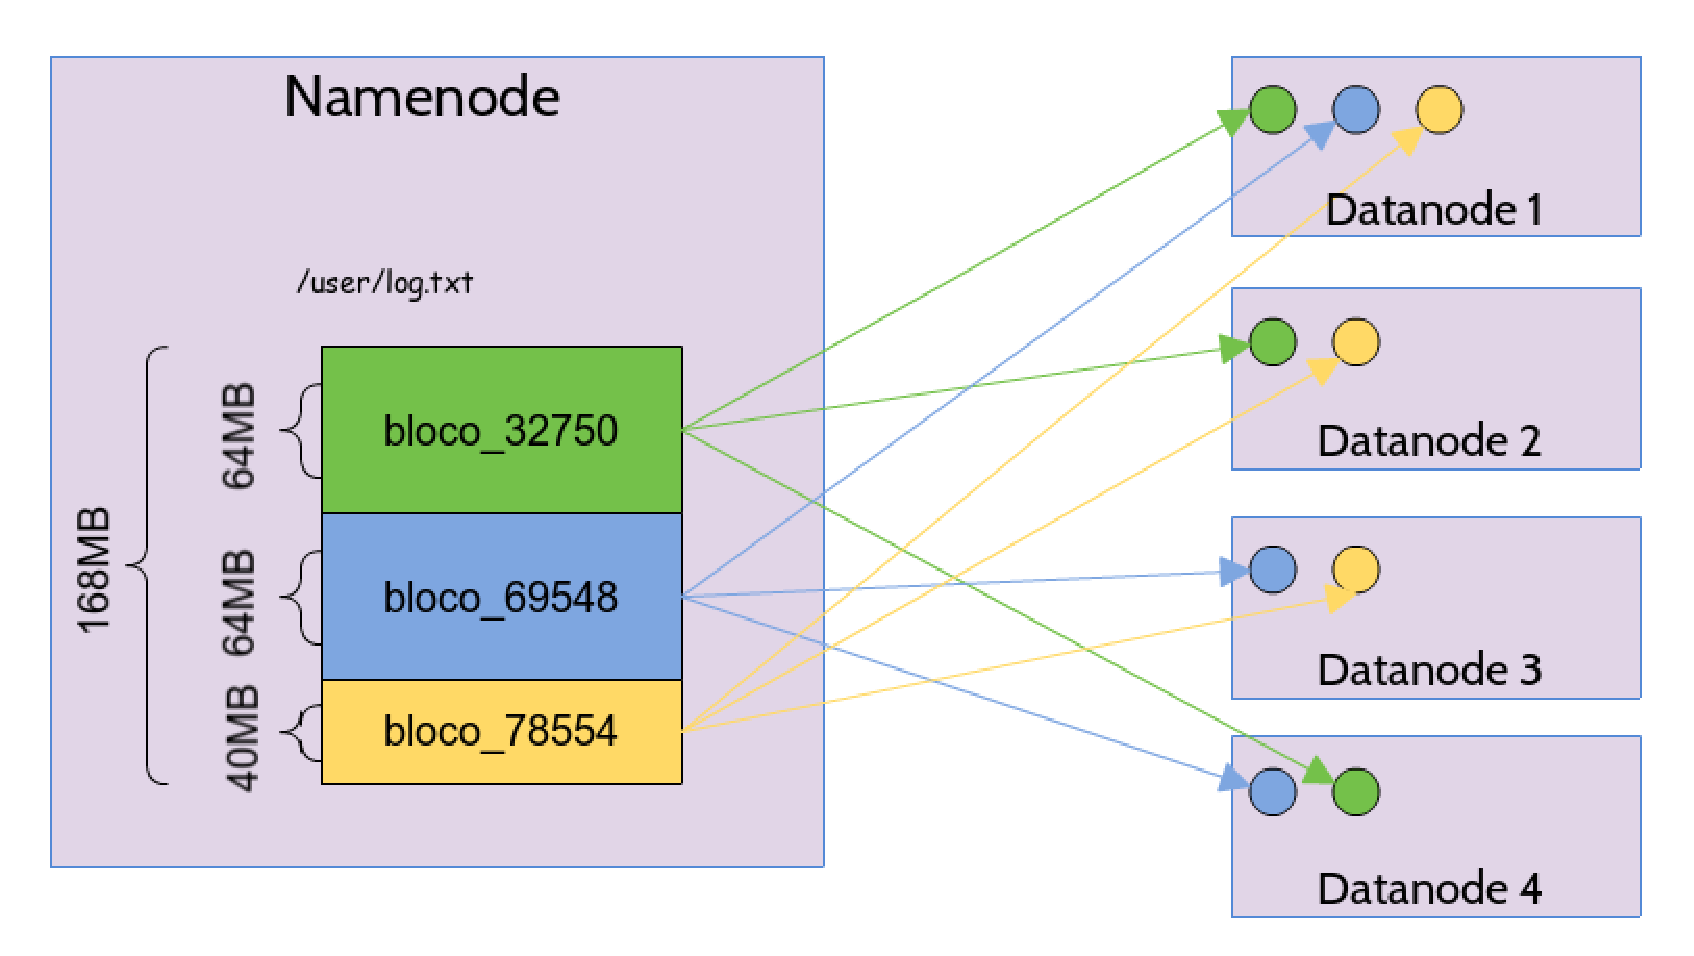
\includegraphics[keepaspectratio=true,scale=0.45]
	  {figuras/hdfs-blocos.eps}
	\caption{Divisão de Arquivos em Blocos}
	\label{fig-hdfs-blocos}
\end{figure}

A utilização de blocos permite simplificar o processo de gerenciamento do armazenamento dos dados. Uma vez que possuem tamanho fixo a tarefa de calcular a quantidade de blocos necessária para todo disco torna-se uma tarefa mais simples. Esta abordagem também permite que blocos sejam replicados pelo sistema de arquivos, provendo tolerância a falhas e uma maior disponibilidade dos dados.

\subsection{Arquitetura}

Um cluster HDFS possui uma arquitetura baseada no modelo mestre/escravo, no qual é composto por um único nó mestre chamado namenode, e um ou mais nós escravos definidos como datanodes. O sistema foi construído utilizando a linguagem de programação java e projetado para ser executado em distribuições GNU/Linux. Portanto para que uma máquina seja um namenode ou datanode é necessário apenas que possua uma JVM disponível juntamente com o sistema operacional adequado.

O namenode é um servidor responsável por gerenciar o namespace do HDFS e também controlar o acesso de clientes aos arquivos contidos no sistema. Este componente mantém a árvore de diretórios e todos os metadados relacionados a ela. Como descrito anteriormente, o HDFS quebra um arquivo em vários blocos e os espalha pelos diversos datanodes do cluster, o namenode possui a tarefa de manter a localização de cada um desses blocos. Todas estas informações são armazenadas no disco local do servidor em dois arquivos: a imagem do sistema de arquivos e o registro de log (WHITE, 2012). O arquivo de imagem do sistema de arquivos também é mantido em memória e é constantemente atualizado.

\begin{figure}[h!]
	\centering
	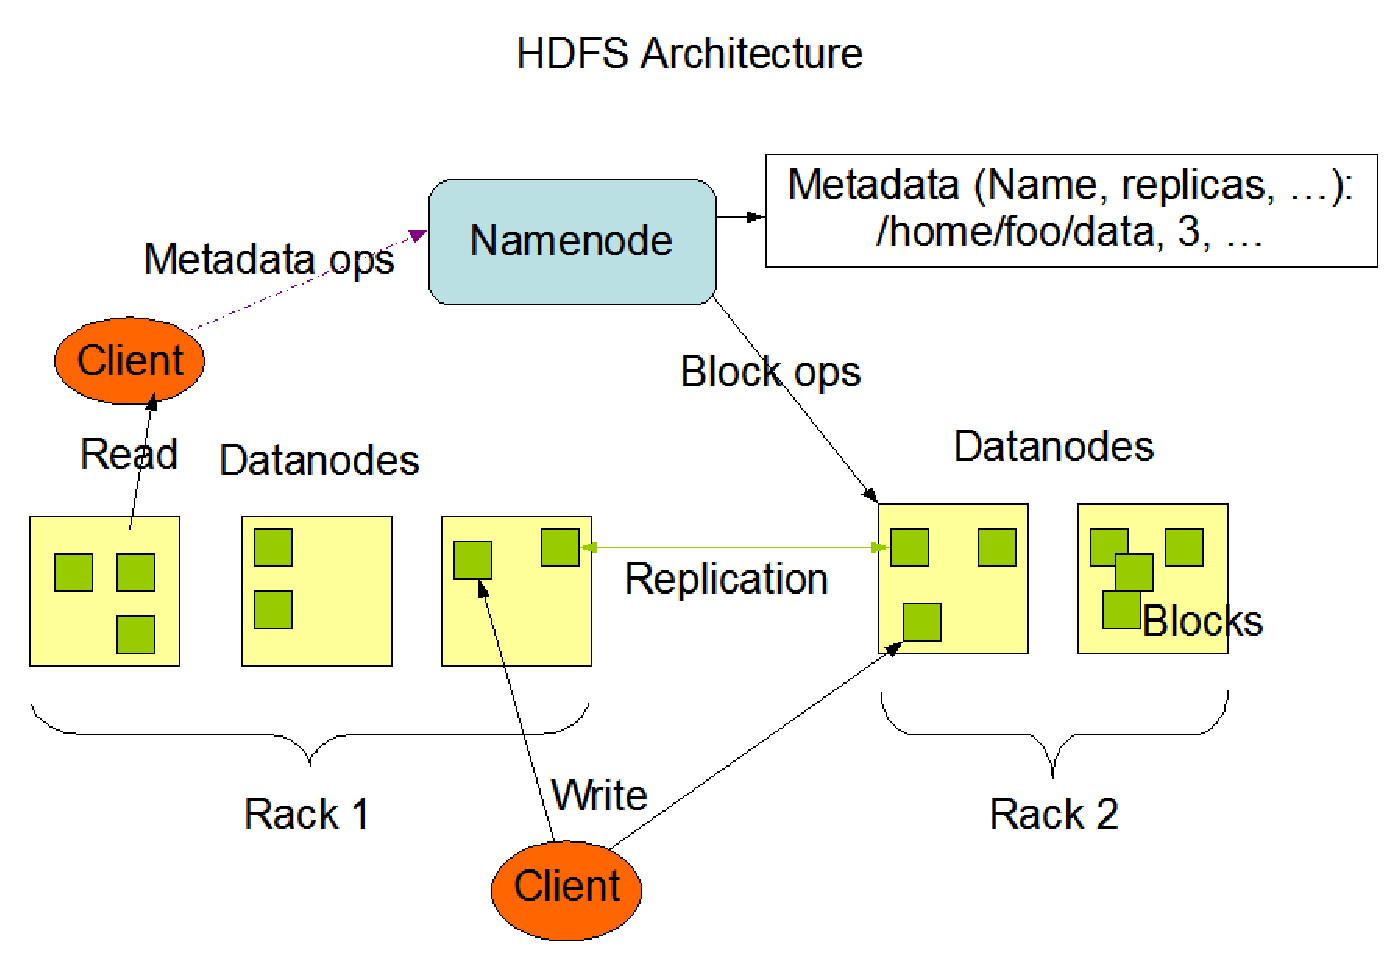
\includegraphics[keepaspectratio=true,scale=0.45]
	  {figuras/hdfs-arquitetura.eps}
	\caption{Arquitetura HDFS}
	\label{fig-hdfs-arquitetura}
\end{figure}

Os datanodes representam os nós escravos do HDFS. Eles são responsáveis por armazenar  fisicamente os blocos de arquivos e recuperá-los quando solicitado pelo namenode. Cada datanode se comunica com o namenode do cluster através da camada de transporte TCP/IP, na qual é utilizada uma abstração do protocolo de chamada remota de procedimento (RPC). Periodicamente os datanodes informam ao namenode quais blocos cada um deles está armazenando.

\section{MapReduce}

MapReduce pode ser definido como um paradigma de programação voltado para processar grandes volumes de dados ao longo de várias máquinas, no qual se utiliza o conceito de programação distribuída para resolver problemas, adotando a estratégia de dividi-los em problemas menores e independentes. O usuário deste modelo define uma função “map”, que deverá processar um par chave-valor e gerar conjuntos intermediários de pares chave-valor, e também uma função “reduce”, responsável por unir  todos os valores intermediários associados a uma mesma chave intermediária (DEAN e GHEMAWAT, 2004)4. Este modelo é baseado no paradigma adotado pela programação funcional e vários problemas reais podem ser resolvidos utilizando esta abordagem. 

Um programa MapReduce separa arquivos de entrada em diversas partes independentes que servem de entrada para as funções map, que executam a mesma tarefa paralelamente. As saídas destas funções são ordenadas por chave-valor e posteriormente transformadas em entradas para a função reduce, onde o resultado final será salvo em um arquivo de saída. Para utilizar este paradigma é necessário apenas se preocupar com as funções map e reduce. Todo gerenciamento dos processos, entre outras questões operacionais são de responsabilidade do framework.

\begin{figure}[h!]
	\centering
	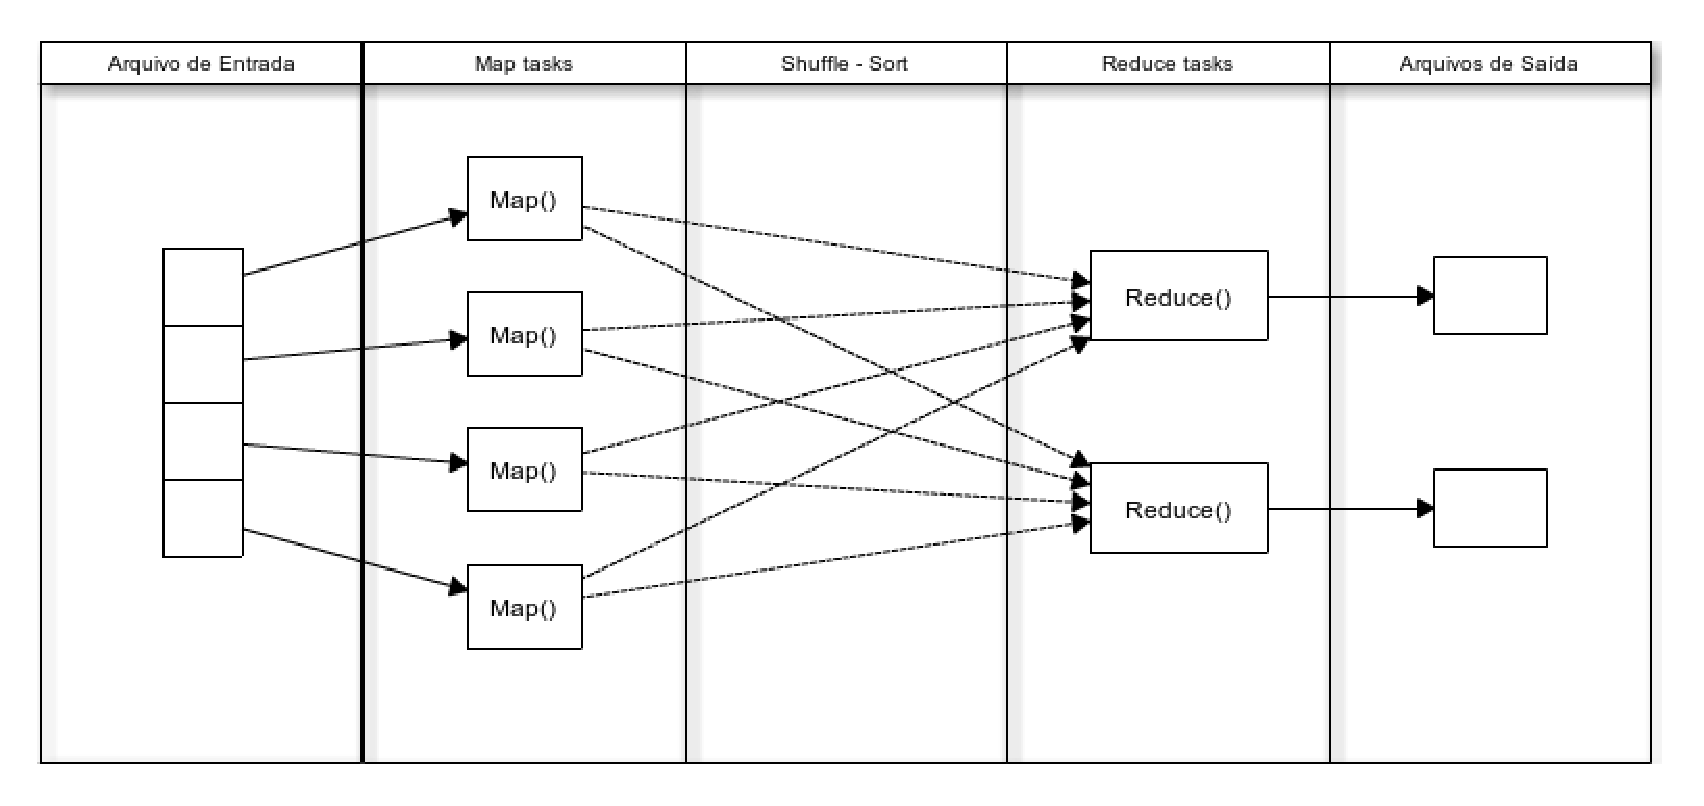
\includegraphics[keepaspectratio=true,scale=0.45]
	  {figuras/mapreduce.eps}
	\caption{MapReduce Job}
	\label{fig-mapreduce}
\end{figure}

\subsection{Contador de Palavras}


Um exemplo simples da aplicabilidade do MapReduce pode ser observado em um problema definido como contador de palavras. Suponha que exista um arquivo de texto com várias palavras inseridas, onde o objetivo seja contar a quantidade de ocorrências de cada uma destas palavras ao longo de todo texto. A princípio parece ser uma atividade trivial, entretanto se o tamanho do arquivo estiver na ordem de gigabytes e aumentarmos a quantidade de arquivos a serem processados o tempo de execução aumentará consideravelmente, tornando-se inviável realizar esta análise.

Uma alternativa para contornar este problema seria o uso da programação paralela, analisando os arquivos em diferentes processos, utilizando quantas threads fossem necessárias. Todavia esta solução não é a mais eficiente, já que os arquivos podem apresentar diferentes tamanhos, ou seja, alguns processos seriam finalizados em um intervalo de tempo menor, impossibilitando maximizar a capacidade de processamento. 

Uma abordagem mais eficiente seria separar todos os arquivos em blocos pré definidos e então dividi-los em processos distintos. Esta solução requer um mecanismo de sincronização complexo e de difícil implementação. Seria necessário agrupar todas as palavras e suas respectivas ocorrências em cada uma das threads nos diferentes processos em execução. E mesmo assim a capacidade de processamento estaria limitada a apenas uma máquina.

Este problema que se mostrou complexo possui uma solução simples e de fácil construção quando utiliza-se a abordagem apresentada pelo paradigma MapReduce. Nesta situação torna-se necessária apenas a definição de uma função map para realizar a contagem de cada palavra presente nos arquivos de entrada, e também de uma função reduce para agrupar cada uma destas palavras e realizar a contagem final dos registros de ocorrências. Todo o trabalho de divisão das entradas em tamanhos fixos e computação distribuída envolvida é realizado pelo framework.

\begin{figure}[h!]
	\centering
	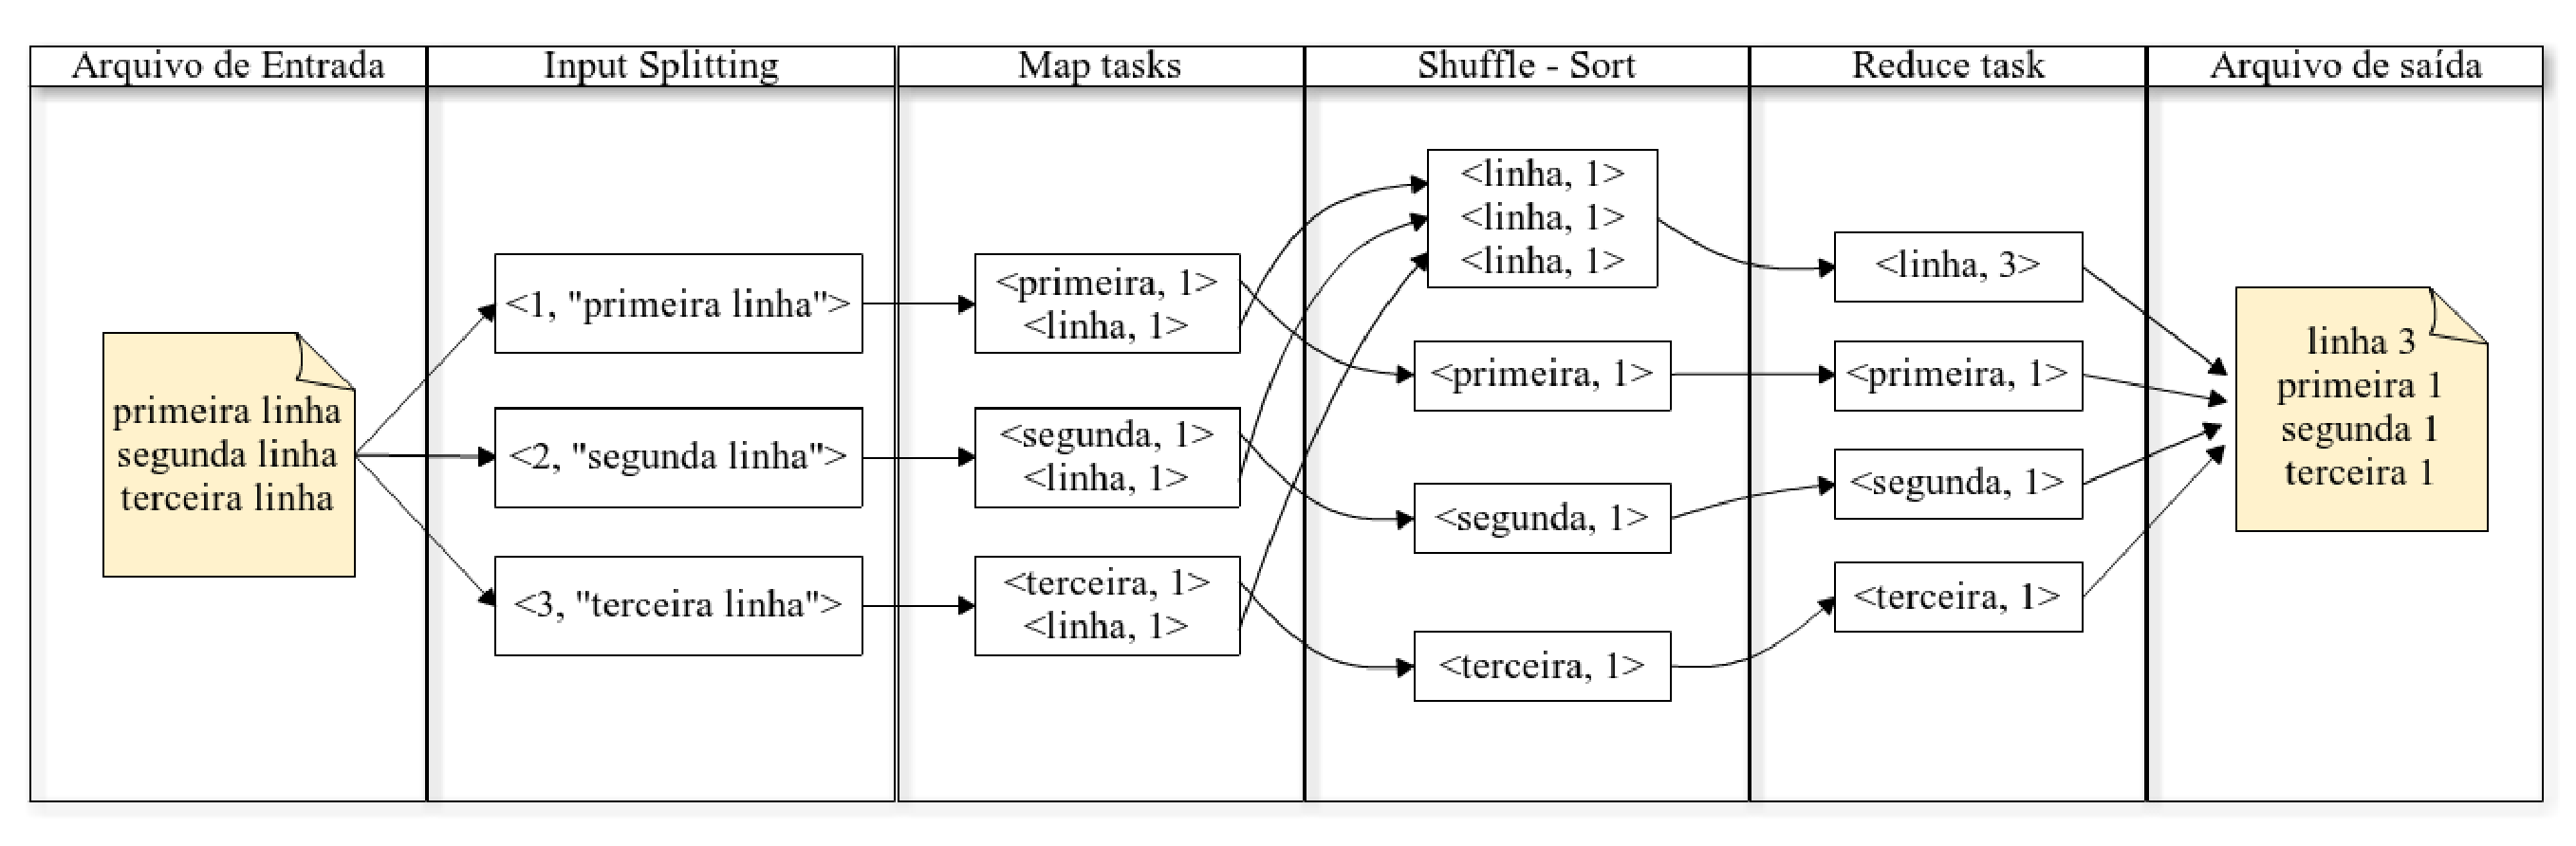
\includegraphics[keepaspectratio=true,scale=0.45]
	  {figuras/mapreduce-word-count.eps}
	\caption{Fluxograma para o job contador de palavras}
	\label{fig-mapreduce-word-count}
\end{figure}

Neste exemplo o programa MapReduce irá dividir todos os arquivos de entrada (armazenados em um sistema de arquivos distribuídos) em um conjunto de linhas, onde cada uma delas será o insumo de uma função map, executada paralelamente em um processo próprio e independente. Esta função é definida pelo usuário e possui apenas o objetivo de registrar uma palavra e atribuir a sua ocorrência o valor 1 (um). Ao término da execução de todas as funções map o framework irá ordenar e agrupar todos os resultados de acordo com as palavras registradas. Cada conjunto agrupado será a entrada para uma função reduce (também definida pelo usário), onde a ocorrência de cada palavra é somada e o resultado final é obtido.

\subsection{Arquitetura}

O framework MapReduce constitui a segunda camada do sistema Hadoop. Para que se realize o processamento de um volume elevado de dados aplicando o conceito de computação distribuída é necessário que os arquivos a serem analisados sejam persistidos em um sistema de arquivos distribuídos. Neste contexto o Hadoop utiliza o HDFS, tornando possível a divisão do trabalho computacional realizado pelo MapReduce ao longo dos nós que armazenam diferentes blocos de arquivos.

Um Mapreduce job é a unidade de trabalho a ser executada por usuários deste modelo e consiste nos arquivos de entrada, no próprio programa MapReduce e também nas informações de configurações. O Hadoop executa este job através de sua divisão em atividades, as quais podem ser do tipo map ou reduce2. A execução destes jobs é realizada por dois tipos de nós: um jobtracker e um conjunto de tasktrackers. 

O jobtracker tem a responsabilidade de coordenar todos os jobs do sistema e também de realizar o agendamento e monitoramento das tarefas a serem executadas pelos tasktrackers. Cada tasktracker executa um conjunto de tarefas determinado pelo jobtracker, o mantendo informado sobre o progresso destas atividades. Caso uma tarefa falhe o jobtracker realizará o reagendamento da mesma para um outro tasktracker, provendo um mecanismo de tolerância a falhas.

Assim como no HDFS a arquitetura do MapReduce é baseada no modelo mestre/escravo, e sua implementação também foi concebida através da linguagem de programação java. Geralmente o namenode e o jobtracker estão localizados no mesmo nó do cluster Hadoop, enquanto cada datanode possui um tasktracker.

\begin{figure}[h!]
	\centering
	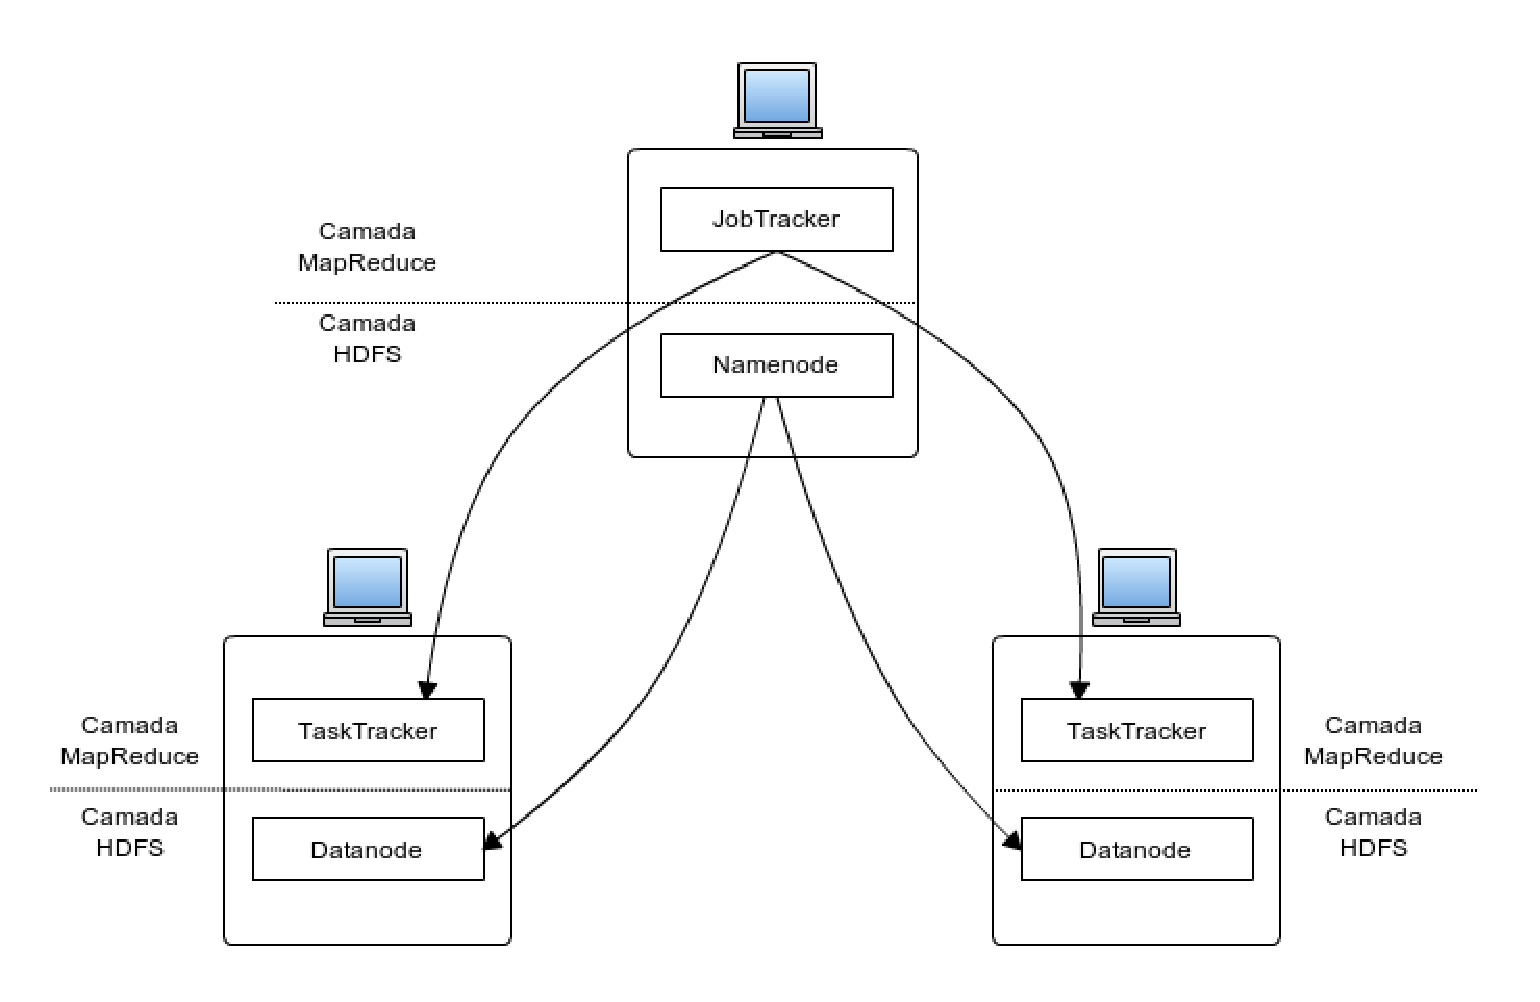
\includegraphics[keepaspectratio=true,scale=0.35]
	  {figuras/mapreduce-arquitetura.eps}
	\caption{Arquitetura MapReduce}
	\label{fig-mapreduce-arquitetura}
\end{figure}

Para realizar a execução de um MapReduce job o Hadoop primeiramente divide os arquivos de entrada em blocos de aproximadamente 64MB, assim como a abordagem utilizada pelo HDFS. Em seguida cada um destes blocos dará origem a uma atividade map, que por sua vez executará a função map (definida pelo usuário) para cada um dos registros presentes em seu respectivo bloco. 

O Hadoop procura executar uma atividade map na mesma máquina onde seu arquivo de entrada está localizado no HDFS. Desta maneira o trabalho computacional é dividido ao longo dos nós do cluster evitando a utilização da rede durante este passo. Cada atividade map escreve seu resultado no próprio disco da máquina e não no HDFS, pois estes arquivos temporários são apenas valores intermediários.

\begin{figure}[h!]
	\centering
	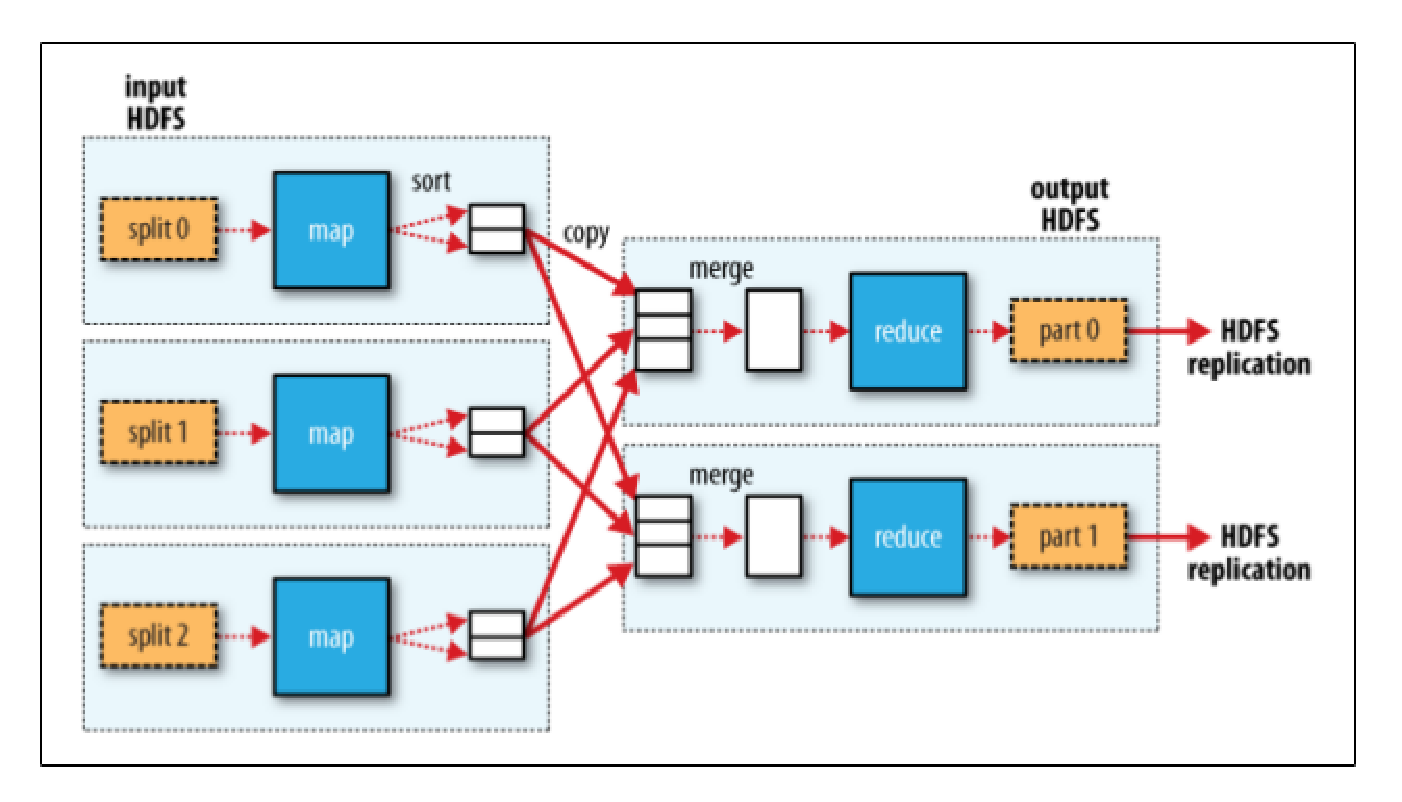
\includegraphics[keepaspectratio=true,scale=0.45]
	  {figuras/mapreduce-job.eps}
	\caption{Fluxograma MapReduce job}
	\label{fig-mapreduce-job}
\end{figure}

As atividades do tipo reduce recebem como entrada os valores intermediários gerados pelas atividades map. Isso significa que estas informações devem ser trasportadas pela rede até a máquina onde estas tarefas reduce serão executadas. Após chegarem ao destino estes dados são agrupados em conjuntos e processadas em atividades reduce distintas, as quais executam a função reduce especificada pelo usuário. O resultado final é salvo em um arquivo no HDFS.


